\documentclass{article}

\usepackage {setspace}
\usepackage [pdftex]{graphicx}
\usepackage[sort&compress]{achemso}

\usepackage[
top    = 1.0in,
bottom = 1.0in]{geometry}

\begin{document}

\newcommand{\suldiox}{SO$_2$}
\newcommand{\ang}{\,$\textrm{\AA}$}
\newcommand{\angs}{\ang}
\newcommand{\wat}{H$_2$O}

\doublespacing

\section* {Supplementary Materials}

The SO$_2$ model used in our simulations was originally parameterized for use with the Dang-Chang water model as used in the work of Baer et al (J. Phys. Chem. B 2010, 114, 7245–7249). In the present work, the POL3 water model was used because of the computational efficiency afforded by the rigid bonds, and the incorporation of the POL3 model into the Amber suite of MD tools that was used for carrying out the simulations. The radial distribution functions of the water-SO$_2$ have been calculated, along with the interaction energy of the H$_2$O-SO$_2$ system as a function of the S-O distance. These are directly comparable to the results of Baer et al. The results are in very good agreement with the Dang-Chang model used with the polarizable SO$_2$, and justify the use of the simpler POL3 model for these interfacial simulations.


\begin{figure}[h!]
	\begin{center}
		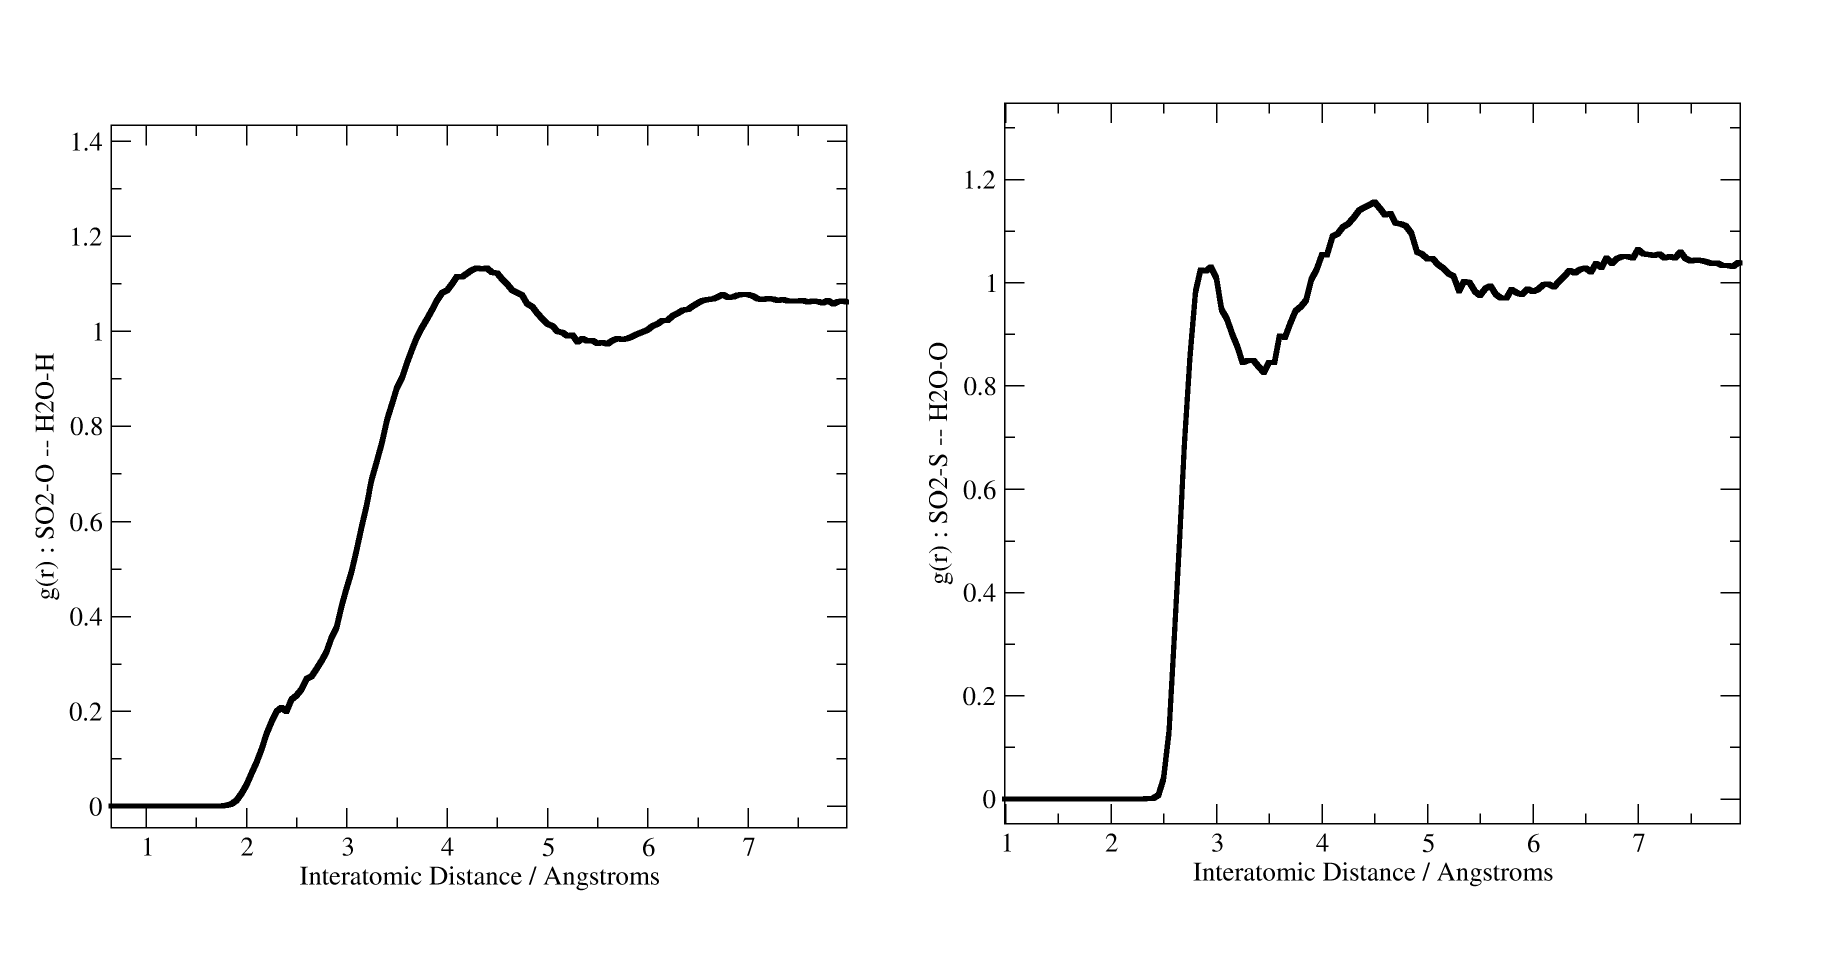
\includegraphics[scale=1.0]{rdf.png}
	\end{center}
\end{figure}

\begin{figure}[h!]
	\begin{center}
		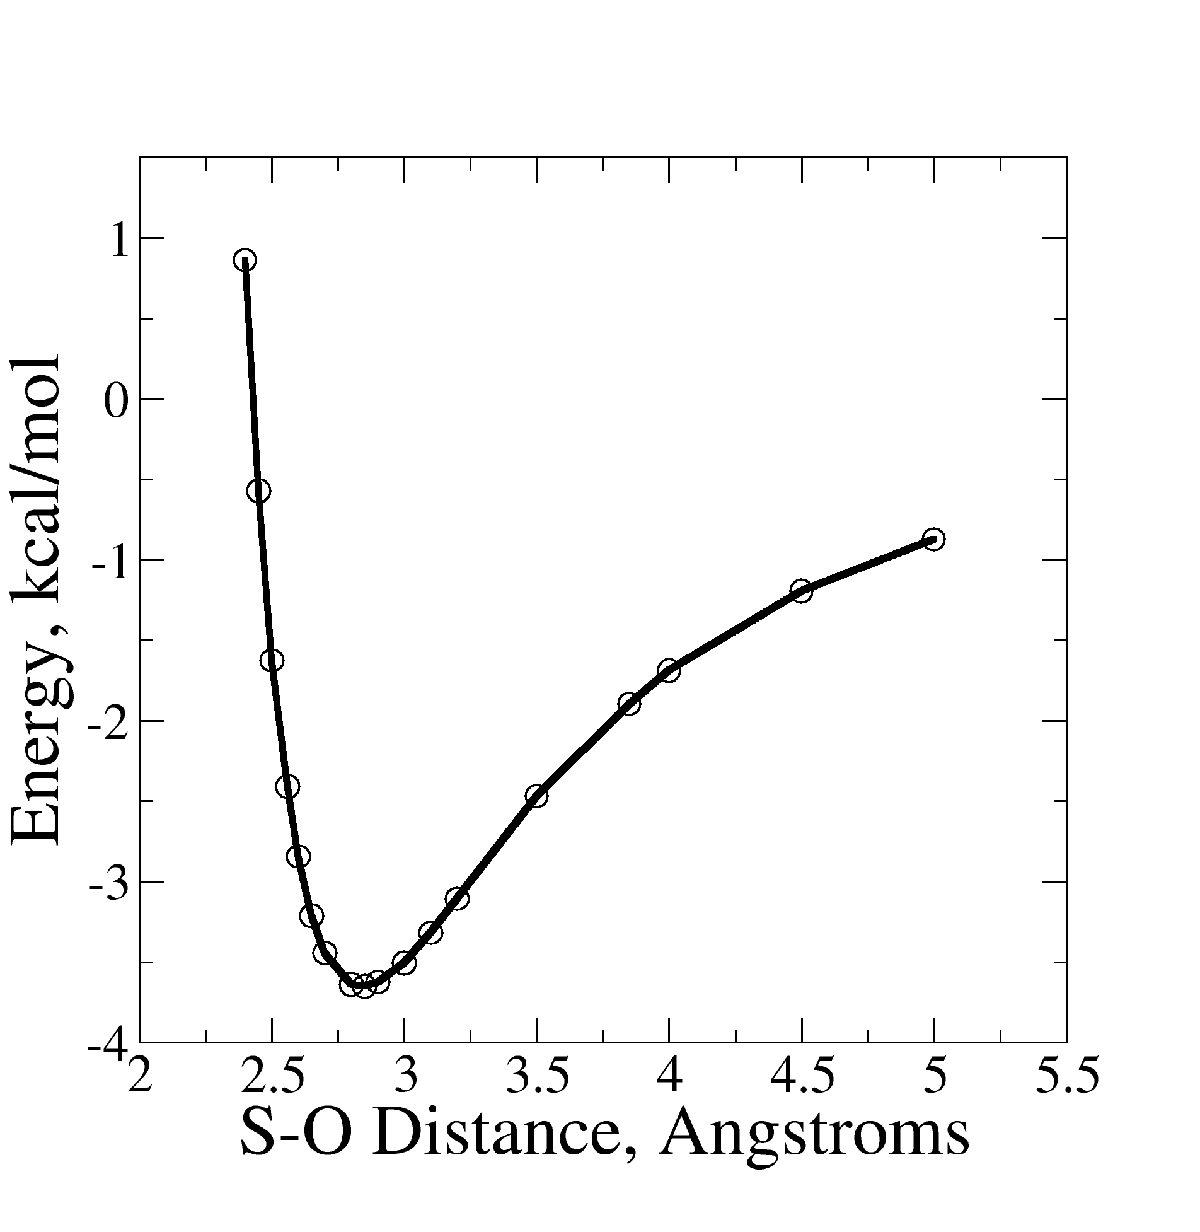
\includegraphics[scale=1.0]{interaction-energy.png}
	\end{center}
\end{figure}

\end{document}
